\section{Results}
In this section we present our results from the experiments. The experiments follow the same order as they were presented in the previous section.


\subsection{Response time distribution}

\clearpage

\begin{figure}[h]
    \centering
    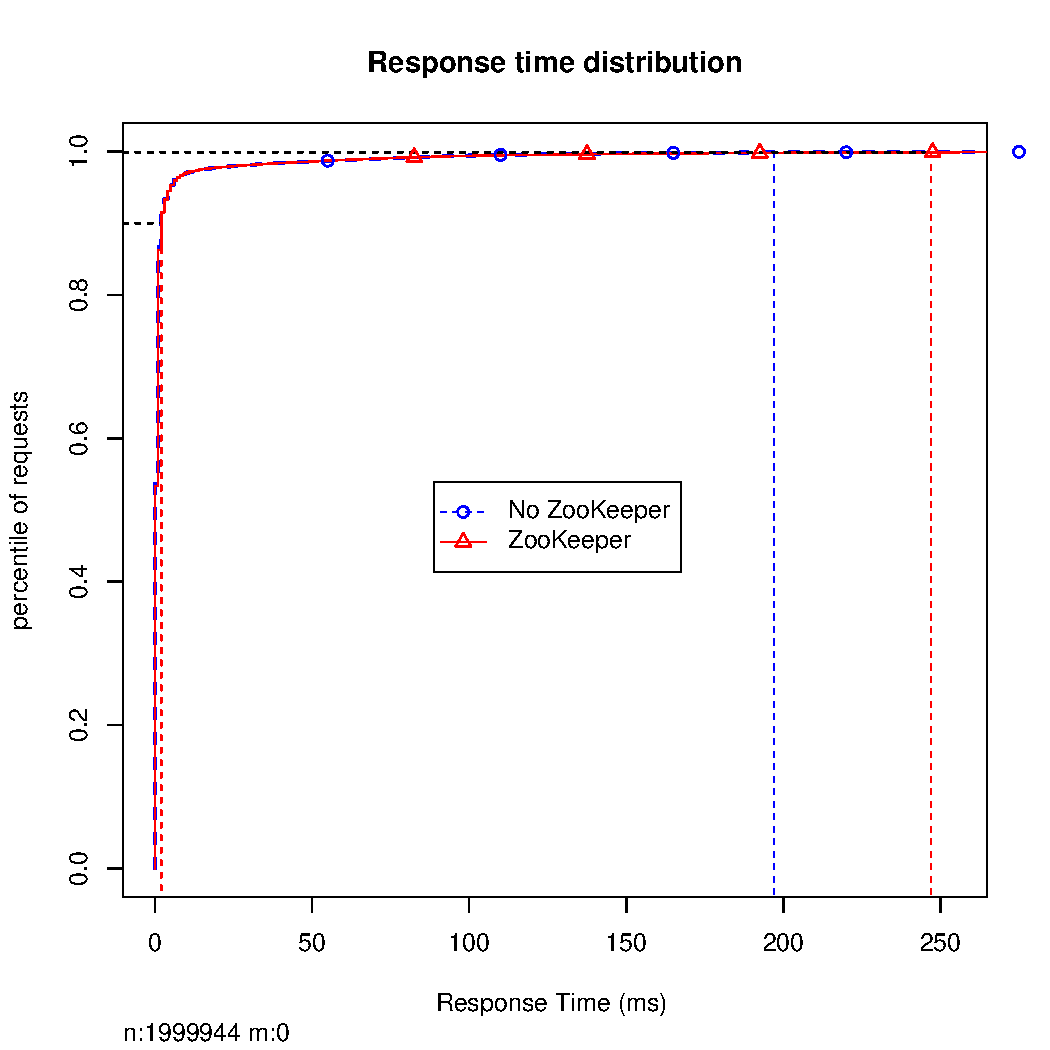
\includegraphics[width=1.0\textwidth]{results/distribution/distribution_macmini}
    \caption{Response time distribution Core 2 Duo Mac mini running both original code and our ZooKeeper implementation}
    \label{fig:dist_mini}
\end{figure}

From Figure \ref{fig:dist_mini} we see that both systems perform similarly on the Mac mini. The vertical lines mark the 0.9 and 0.999 percentile of requests. We see that 90\% of the requests are serviced within 2 ms while at the .999 percentile the response time is at 197 ms for our implementation and 247 ms for the original code.  

\clearpage

\begin{figure}[h]
    \centering
    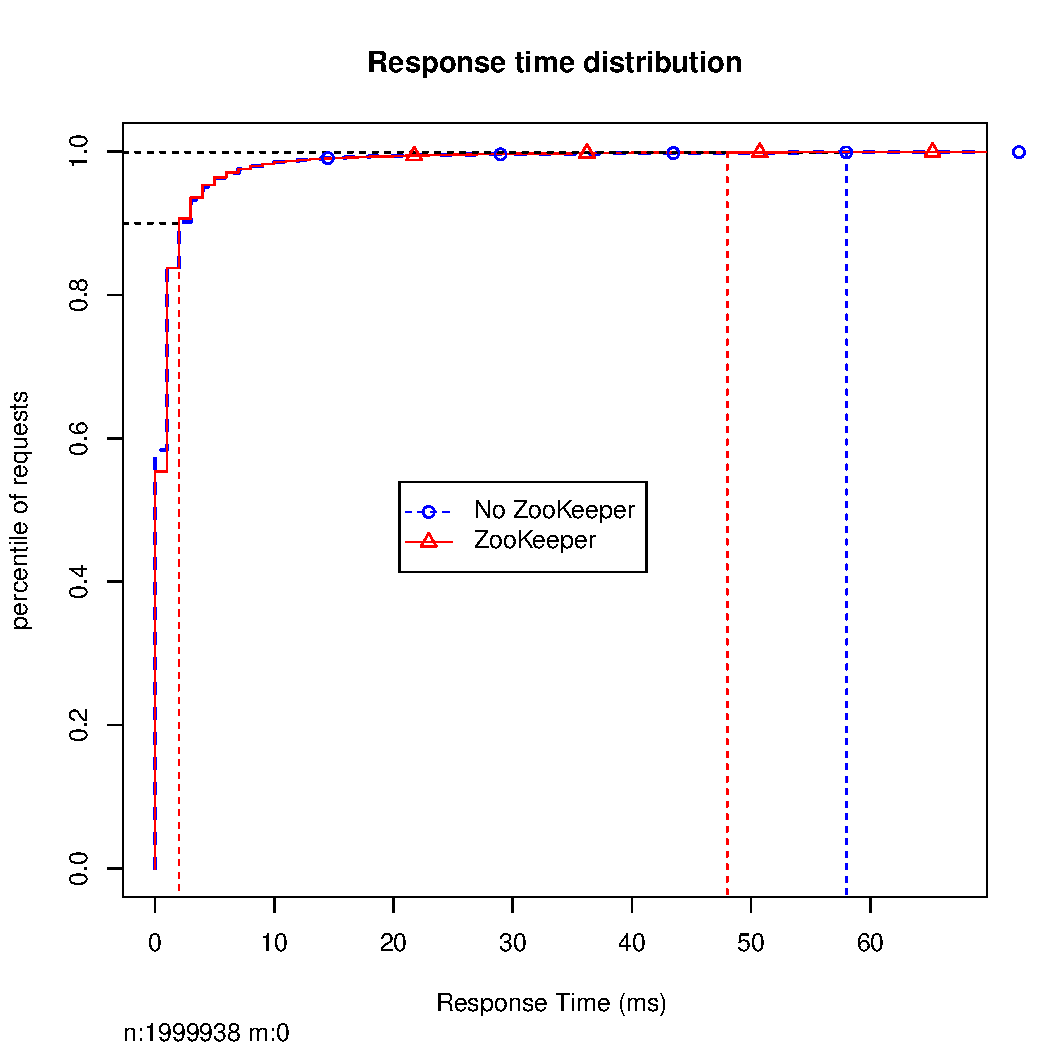
\includegraphics[width=1.0\textwidth]{results/distribution/distribution_knut}
    \caption{Response time distribution i5 MacBook running both original code and our ZooKeeper implementation}
    \label{fig:dist_knut}
\end{figure}

From Figure \ref{fig:dist_knut} we see that both systems still perform similarly on the i5 MacBook Pro. The vertical lines again mark the 0.9 and 0.999 percentile of requests. At the 0.90 percentile we see no improvement, however at the 0.999 percentile we see a massive improvement with 58 ms on our ZooKeeper implementation and 48 ms on the original code.  

\clearpage

\begin{figure}[h]
    \centering
    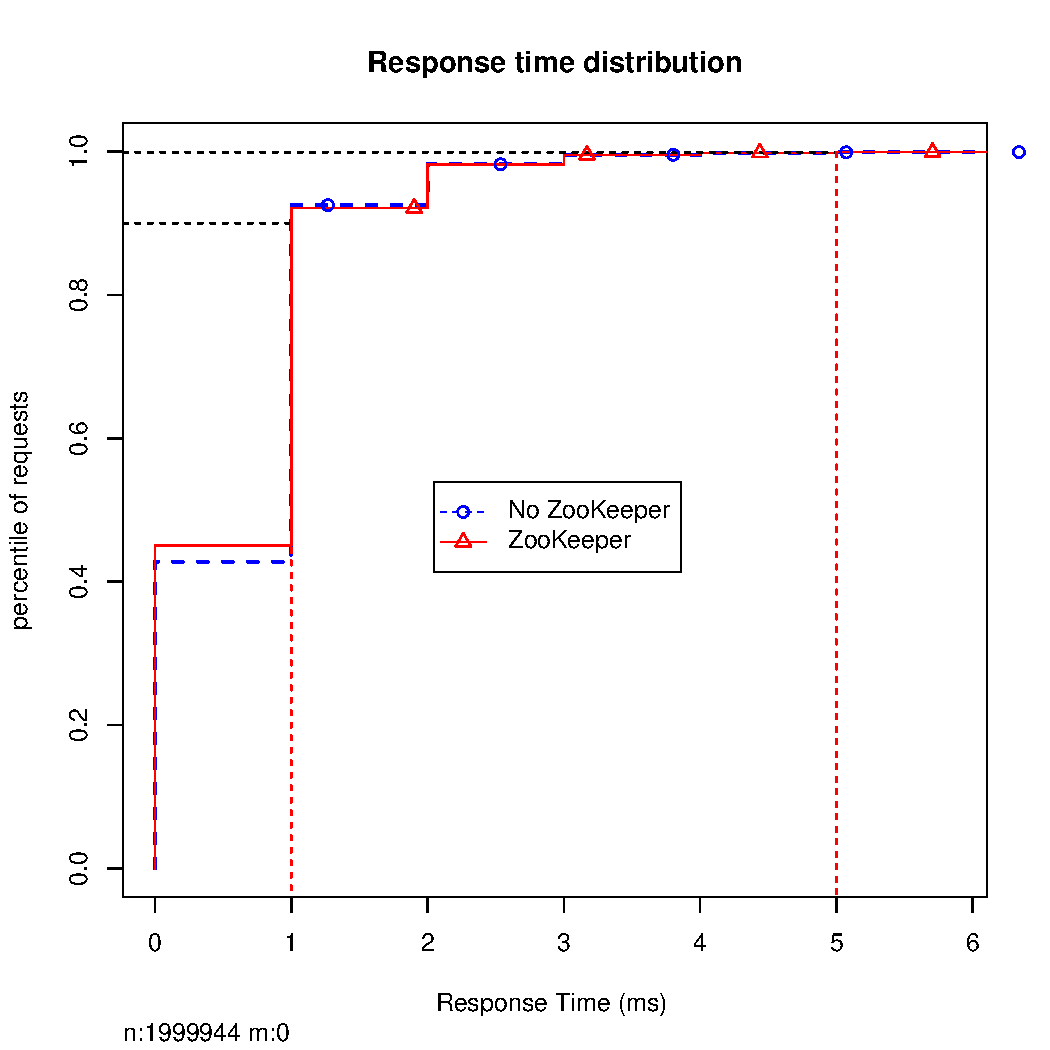
\includegraphics[width=1.0\textwidth]{results/distribution/distribution_eivind}
    \caption{Response time distribution i7 MacBook running both original code and our ZooKeeper implementation}
    \label{fig:dist_eivind}
\end{figure}

Finally in Figure \ref{fig:dist_eivind} we see the results on the i7 Macbook Pro. Again we see both implementations of Voldemort performing equally. At the 0.90 percentile the system responds in 1 ms in both cases and again we see a great increase in performance at the 0.999 percentile with 5 ms for both systems.

\subsection{Throughput}

\clearpage

\begin{figure}[h]
    \centering
    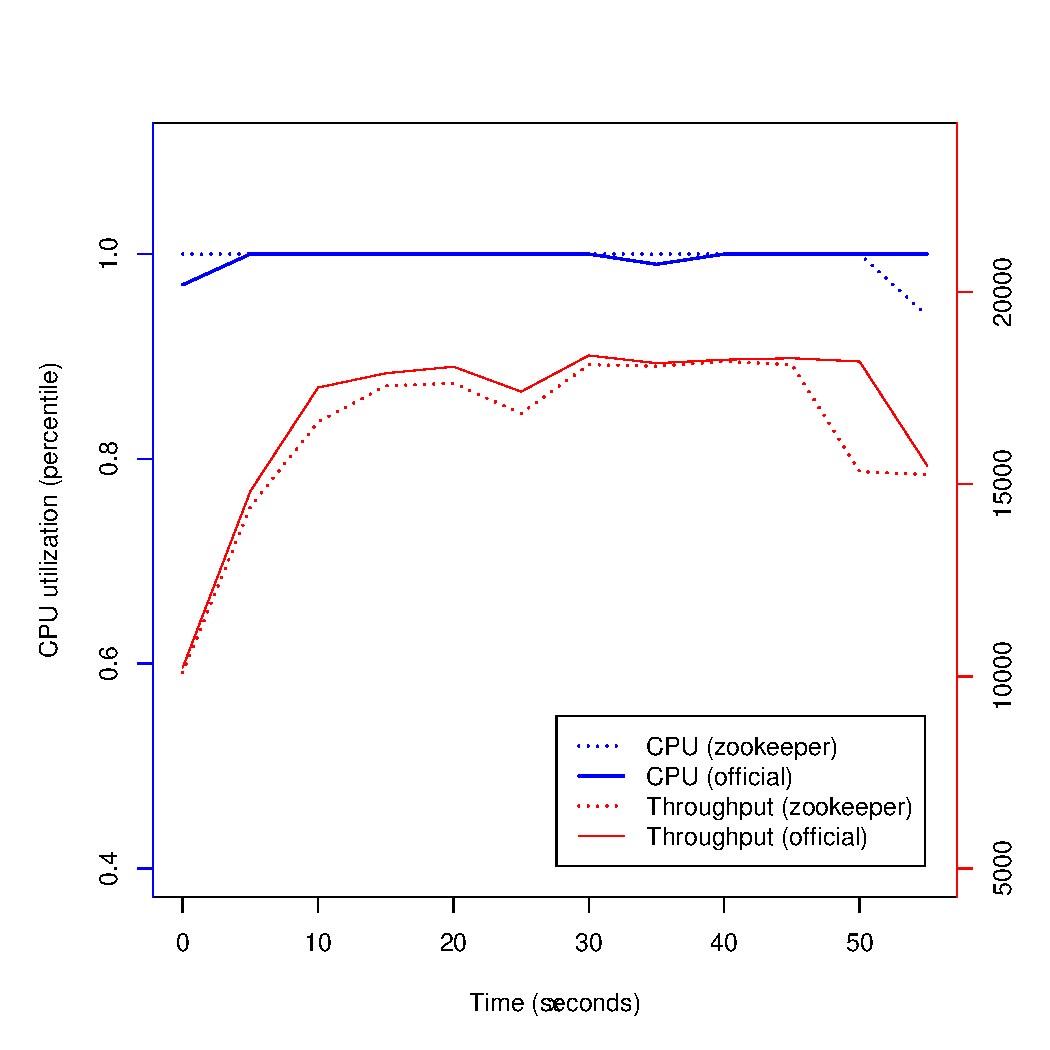
\includegraphics[width=1.0\textwidth]{results/throughput/singlenode/throughput_macmini}
    \caption{Throughput and CPU-load under stress test on Mac Mini}
    \label{fig:thug_mini}
\end{figure}

From Figure \ref{fig:thug_mini} we see that the Mac minis core 2 duo is clearly maxed out keeping up with the workload, running at close to 100\% utilization of the CPU. Maximum throughput seems to hover around 17 000 requests per second.  

\clearpage

\begin{figure}[h]
    \centering
    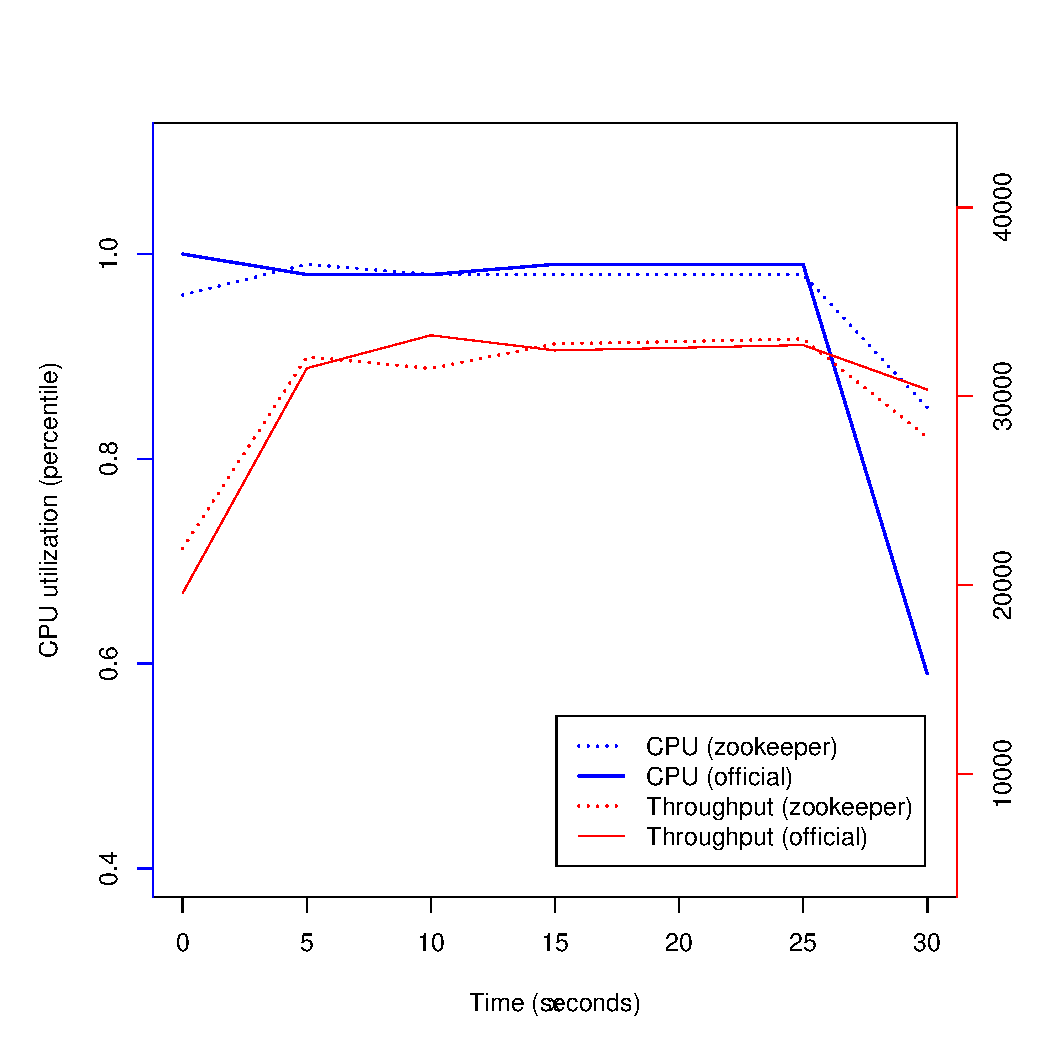
\includegraphics[width=1.0\textwidth]{results/throughput/singlenode/throughput_knut}
    \caption{Throughput and CPU-load under stress test on i5 MacBook Pro}
    \label{fig:thug_knut}
\end{figure}

We see on Figure \ref{fig:thug_knut} that the Core i5 in the MacBook performs a lot better than the Core 2 duo in the mini. The MacBook is still not able to keep up with the work being sent to it, however it is able to serve around 32000 requests per second. 

\clearpage

\begin{figure}[h]
    \centering
    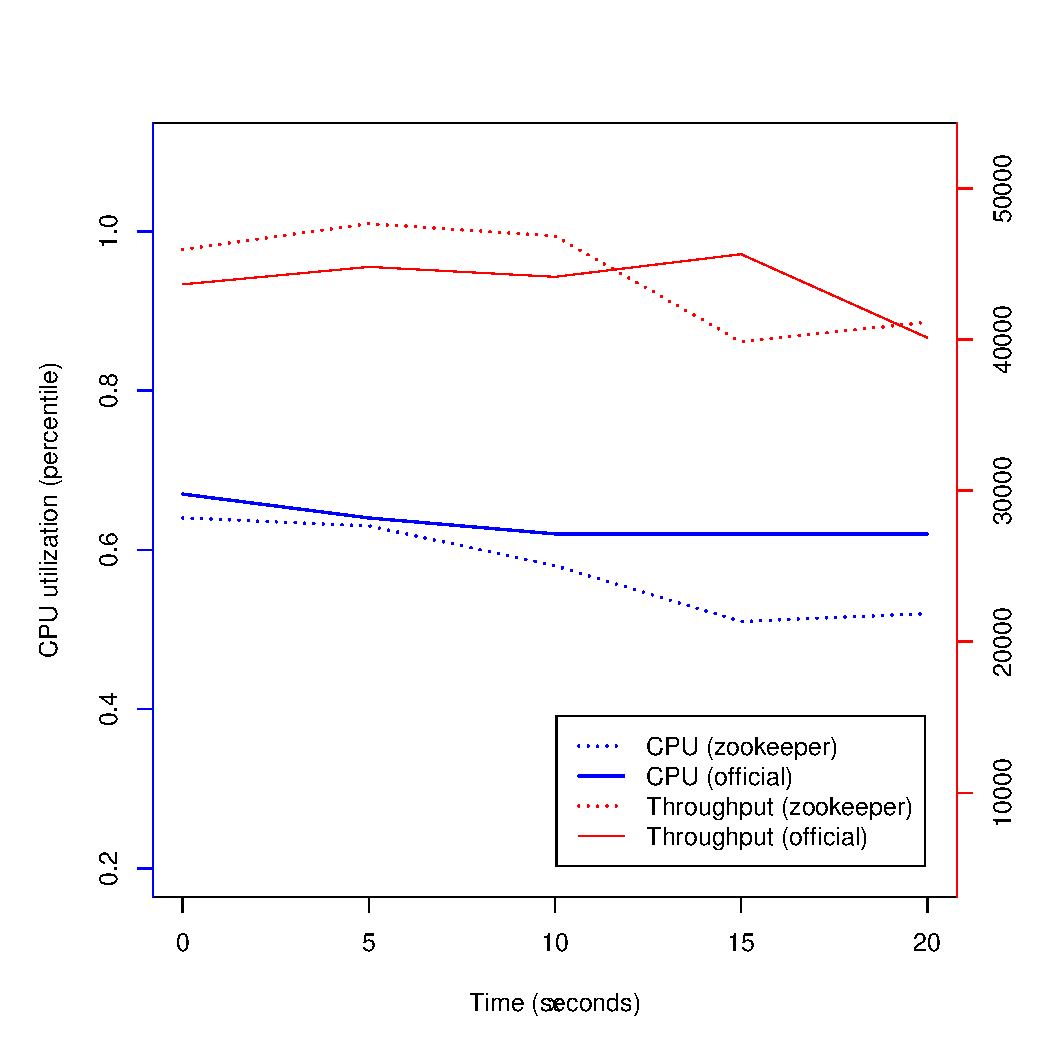
\includegraphics[width=1.0\textwidth]{results/throughput/singlenode/throughput_eivind}
    \caption{Throughput and CPU-load under stress test on i7 MacBook Pro}
    \label{fig:thug_eivind}
\end{figure}

Finally we have the Core i7 Macbook. In Figure \ref{fig:thug_eivind} we see that the Core i7 caps out at around 44000 requests per second. This is the first test where we see that CPU-utilization is not maxed out indicating that disk access might be an limiting factor. 

\subsection{Preliminary findings}
We did not have access to a lot of different hardware while doing this project. Our computers proved quite fast, with each individual node pushing 50-70 MB per second. This made us quickly reach the network speed limit in our benchmarking system, receiving over 130MB/s second from the cluster while benchmarking. This limit was reached around 60k requests/s, so this is our practical, and theoretical, maximum throughput of 1024 kB values. On a 100mbit connection we could only send or receive about 5k requests/s, or roughly 12 MB/s. 

While testing, we noticed no real difference between a 12MB and 2GB cache size on our Voldemort systems. This might suggest there is a problem with the setting in the software. All of our hardware run on SSDs, but we still consider this result surprising. There could be more work done here on largely different sizes of data sets, but this was not our main focus.

Overall while benchmarking we found performance to be very consistent. Our results were on large very reproducible and saw little variance between benchmark runs.

From our initial tests we alse have found no significant difference in the performance between our ZooKeeper implementation and the original Voldemort code. Contrary to our expectations, the response time distribution varies greatly on different hardware. In our results the 0.999 percentile response time varies from 250 ms on the slowest hardware to 5 ms on the fastest. On the .90 percentile there is however is much less difference with response times of 2 ms on the slowest hardware and 1 ms on the fastest.

When it comes to the single node throughput benchmarks the results are more in line with what we expected. The slow Core 2 Duo is barely able to serve 17000 requests per second while the Core i5 and i7 are able to serve 32000 and 44000. With our theoretical limit of 60 000 requests per second we can expect a cluster consisting of the two slower machines to be unable to service a full workload, while a cluster with all 3 nodes should comfortably do so. This information is useful for structuring our adaptive cluster experiments.

\clearpage
\subsection{Adaptive cluster behavior}
In this section follows the results form our adaptive cluster experiments.

\clearpage
\begin{figure}[h]
    \centering
    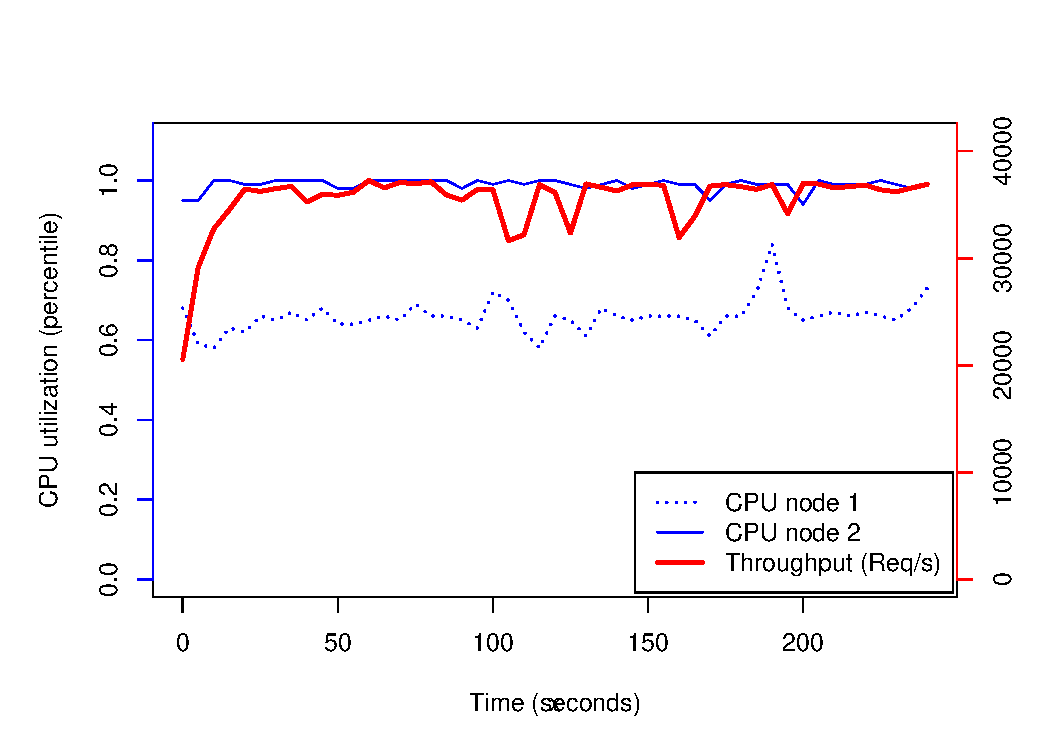
\includegraphics[width=1.2\textwidth]{results/baseline_slowpro_mini}
    \caption{A cluster of 2 nodes serving queries.}
    \label{fig:adaptive_base}
\end{figure}


\clearpage
\begin{figure}[h]
    \centering
    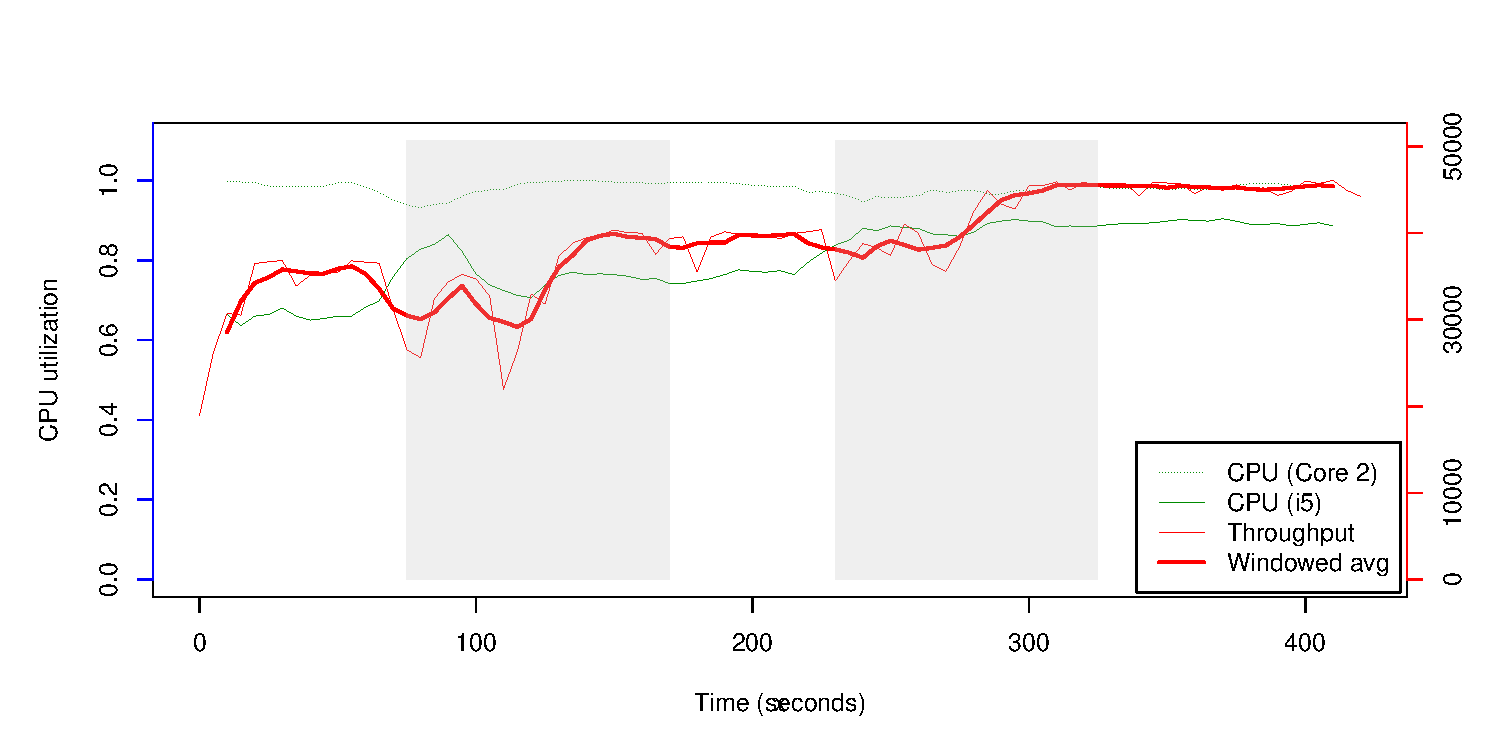
\includegraphics[width=1.2\textwidth]{results/rebalance_manual_2node}
    \caption{Manual moving of 2 partitions from a struggling node (Core 2). Grey regions mark rebalance period, where data is prepared and transferred.}
    \label{fig:adaptive_man}
\end{figure}

In Figure\ref{fig:adaptive_man} we see 2 manual rebalances. We see total CPU-utilization increase as we move partitions away from a struggling node and over to one less worked. The aim of this experiment was to get a baseline to compare our automatic rebalance service to. We see throughput steadily increase after each rebalance moving from around 36k up to 45k. During the rebalance we have two very distict drops in throughput. The first one is from when request starts being proxied and all client threads must reconnect. The second one is from the actual data transfer. 

\clearpage
\begin{figure}[h]
    \centering
    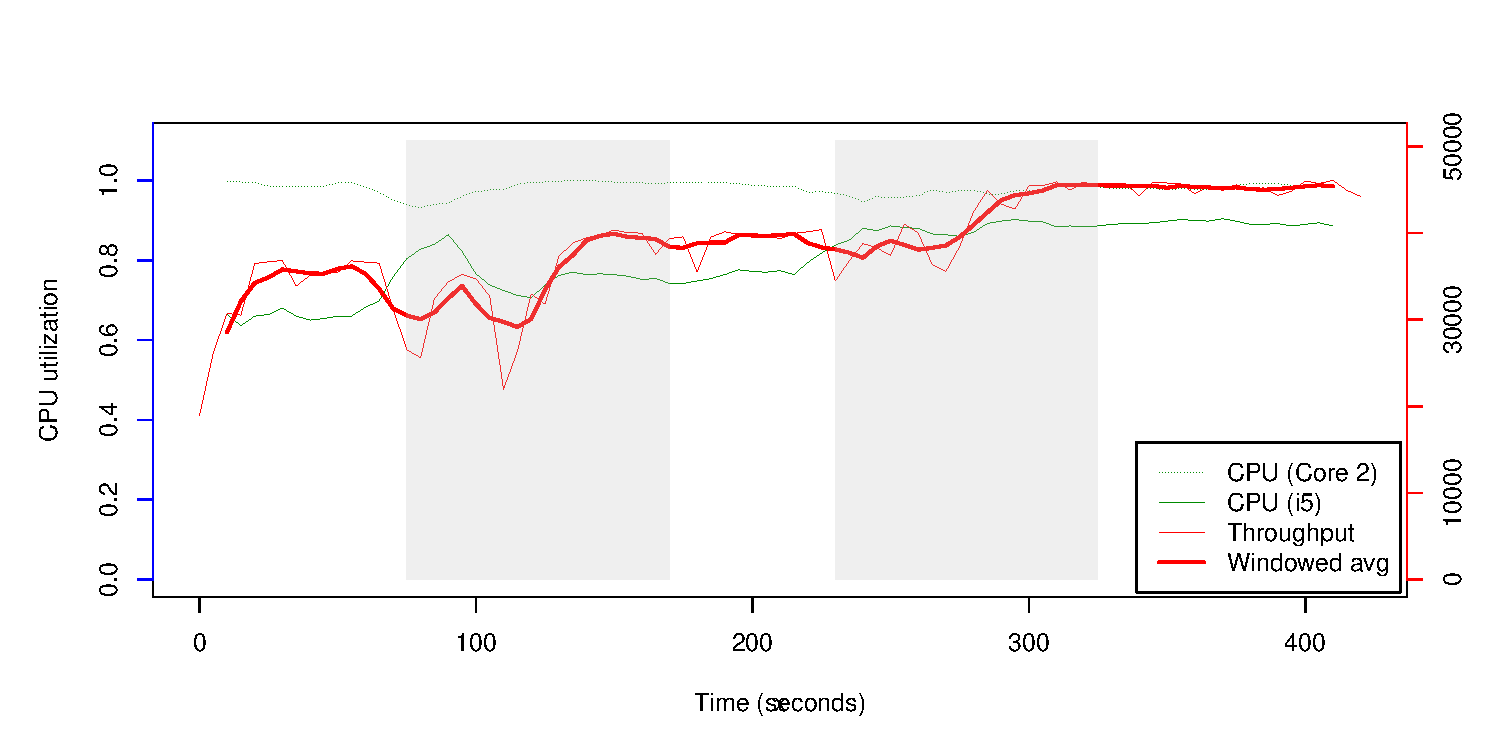
\includegraphics[width=1.2\textwidth]{results/rebalance_auto_2node}
    \caption{Automatic moving of 2 partitions from a struggling node (Core 2). Grey regions mark rebalance period, where data is prepared and transferred. CPU threshold set at \texttt{0.84}.}
    \label{fig:adaptive_auto}
\end{figure}
Figure\ref{fig:adaptive_auto} shows the same experiment just automated by Headmaster. We again see a steady increase in throughput as partitions are moved. This shows that our automatic rebalancer performs just as well as the manual tool in Voldemort.  

\clearpage
\begin{figure}[h]
    \centering
    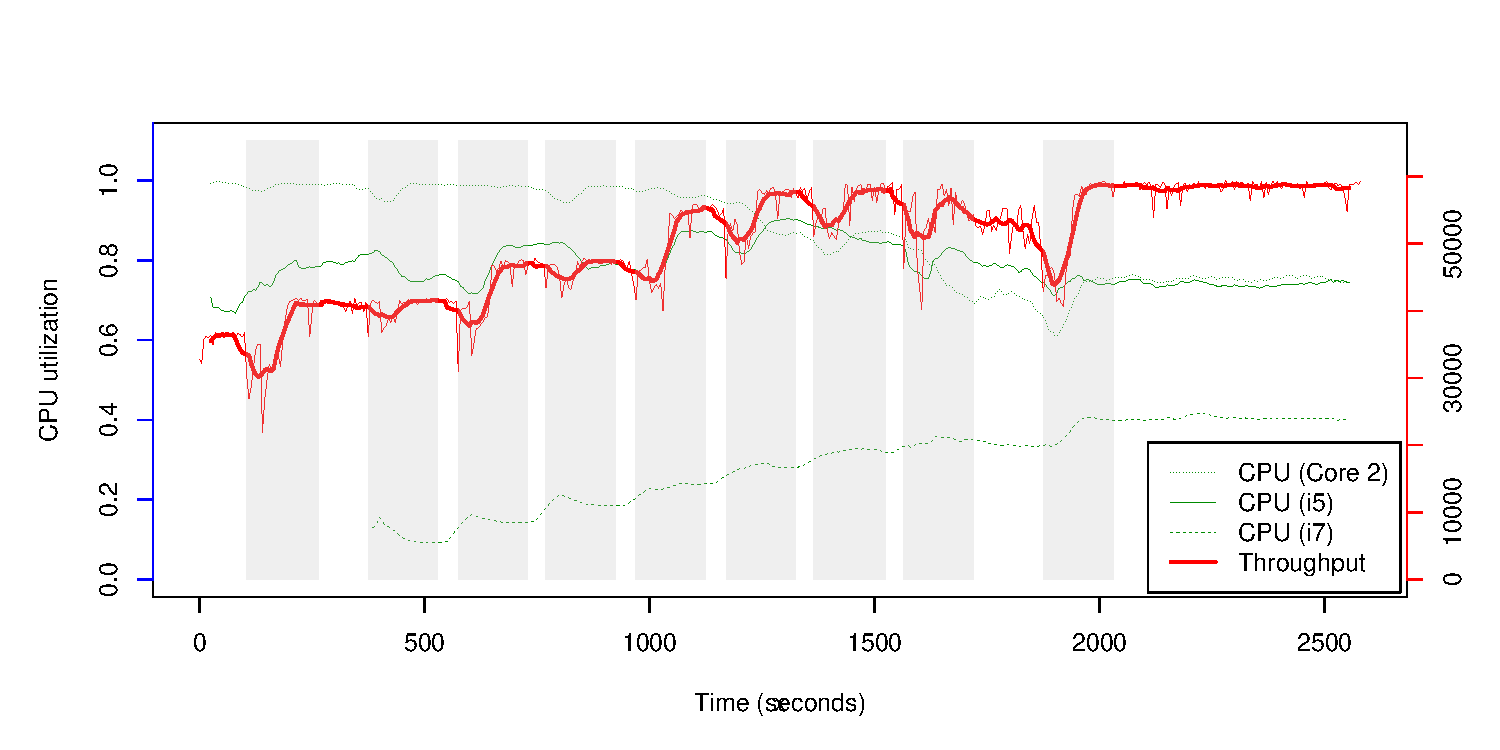
\includegraphics[width=1.0\textwidth]{results/adaptive3node}
    \caption{Automatic migration of partitions in a struggling cluster after a third node joins}
    \label{fig:adapt_3node}
\end{figure}
Our final Figure\ref{fig:adapt_3node} shows the result adding a node to a struggling cluster and rebalance live. At t=380 the i7 is introduced to the cluster. We see a steady increase in performance as more and more partitions are moved to the i7. In the end the partition distribution is 3,6,9 for the Core 2, i5 and i7. 

At t=1700 there is a significant loss of throughput after a rebalance. We found no reason for this in our logs, so we expect this to be related to unrelated work done by the operating system on the workload generating computer. 

\subsection{Adaptive cluter finding}
In our adaptive cluster experiments we have compared automated to manual rebalancing and found our automatic solution to perform on par with the manual one. We have also done a extensive cluster expansion test and monitored CPU-utilization and throughput. These experiments show that our implementation works as intended.





